\documentclass[12pt,]{article}
\usepackage{lmodern}
\usepackage{amssymb,amsmath}
\usepackage{ifxetex,ifluatex}
\usepackage{fixltx2e} % provides \textsubscript
\ifnum 0\ifxetex 1\fi\ifluatex 1\fi=0 % if pdftex
  \usepackage[T1]{fontenc}
  \usepackage[utf8]{inputenc}
\else % if luatex or xelatex
  \ifxetex
    \usepackage{mathspec}
  \else
    \usepackage{fontspec}
  \fi
  \defaultfontfeatures{Ligatures=TeX,Scale=MatchLowercase}
\fi
% use upquote if available, for straight quotes in verbatim environments
\IfFileExists{upquote.sty}{\usepackage{upquote}}{}
% use microtype if available
\IfFileExists{microtype.sty}{%
\usepackage{microtype}
\UseMicrotypeSet[protrusion]{basicmath} % disable protrusion for tt fonts
}{}
\usepackage[margin=1in]{geometry}
\usepackage{hyperref}
\PassOptionsToPackage{usenames,dvipsnames}{color} % color is loaded by hyperref
\hypersetup{unicode=true,
            pdftitle={A TITLE: Keep it simple, brief and attractive},
            colorlinks=true,
            linkcolor=blue,
            citecolor=Blue,
            urlcolor=Blue,
            breaklinks=true}
\urlstyle{same}  % don't use monospace font for urls
\usepackage{graphicx,grffile}
\makeatletter
\def\maxwidth{\ifdim\Gin@nat@width>\linewidth\linewidth\else\Gin@nat@width\fi}
\def\maxheight{\ifdim\Gin@nat@height>\textheight\textheight\else\Gin@nat@height\fi}
\makeatother
% Scale images if necessary, so that they will not overflow the page
% margins by default, and it is still possible to overwrite the defaults
% using explicit options in \includegraphics[width, height, ...]{}
\setkeys{Gin}{width=\maxwidth,height=\maxheight,keepaspectratio}
\IfFileExists{parskip.sty}{%
\usepackage{parskip}
}{% else
\setlength{\parindent}{0pt}
\setlength{\parskip}{6pt plus 2pt minus 1pt}
}
\setlength{\emergencystretch}{3em}  % prevent overfull lines
\providecommand{\tightlist}{%
  \setlength{\itemsep}{0pt}\setlength{\parskip}{0pt}}
\setcounter{secnumdepth}{0}
% Redefines (sub)paragraphs to behave more like sections
\ifx\paragraph\undefined\else
\let\oldparagraph\paragraph
\renewcommand{\paragraph}[1]{\oldparagraph{#1}\mbox{}}
\fi
\ifx\subparagraph\undefined\else
\let\oldsubparagraph\subparagraph
\renewcommand{\subparagraph}[1]{\oldsubparagraph{#1}\mbox{}}
\fi

%%% Use protect on footnotes to avoid problems with footnotes in titles
\let\rmarkdownfootnote\footnote%
\def\footnote{\protect\rmarkdownfootnote}

%%% Change title format to be more compact
\usepackage{titling}

% Create subtitle command for use in maketitle
\newcommand{\subtitle}[1]{
  \posttitle{
    \begin{center}\large#1\end{center}
    }
}

\setlength{\droptitle}{-2em}
  \title{A TITLE: Keep it simple, brief and attractive}
  \pretitle{\vspace{\droptitle}\centering\huge}
  \posttitle{\par}
  \author{}
  \preauthor{}\postauthor{}
  \date{}
  \predate{}\postdate{}

% %\usepackage{helvet}
% %\renewcommand{\familydefault}{\sfdefault}
% 
 %Options: Sonny, Lenny, Glenn, Conny, Rejne, Bjarne, Bjornstrup for chapter layout
\usepackage[Sonny]{fncychap}
\usepackage{refcount}
\usepackage{mathspec}
\usepackage{multirow}
\usepackage{booktabs}
\usepackage{lscape}

\newcommand{\blandscape}{\begin{landscape}}
\newcommand{\elandscape}{\end{landscape}}
\usepackage{caption}
% \usepackage{fontspec}
 %\usepackage[skip=12pt,font=scriptsize]{caption}
 \setmainfont{Arial}
 \usepackage{ragged2e}
 \usepackage{float}

 \usepackage{graphicx}
\usepackage{setspace} %%for equation space
%\numberwithin{equation}{section}
 \usepackage{placeins}
 \usepackage{chngcntr}
 \usepackage{microtype}
 
 
%remove hyphens in latex 
\usepackage[none]{hyphenat}

%\counterwithin{equation}{section} defining the sections for equations
\renewcommand{\theequation}{Eqn:\arabic{equation}}

%setting caption to top
%\usepackage{floatrow}
%\floatsetup[table]{capposition=top}
 \floatstyle{plaintop}
\restylefloat{table}



%https://tex.stackexchange.com/questions/164640/customize-equation-numbering-for-equation-environment
%\usepackage{pdfpages}
%\fontsize{12pt} {}\selectfont
% %\usepackage{bibentry}
% %\bibliography{bibliography.bib}
% %\usepackage{biblatex}
% %\renewcommand*{\bibfont}{\tiny}
% 
\usepackage{fancyhdr}
\pagestyle{fancy}
\fancyhead[R]{\leftmark }
% \fancyhead[R]{KM Wambui - 1504769}
%\fancyfoot[LE,RO]{\thepage}
%\fontsize{14}{22}
%\fontseries{b}
%\selectfont
%\usepackage{setspace}
%\doublespacing


\counterwithin{figure}{section}
\counterwithin{table}{section}

\begin{document}
\maketitle

\large
\setstretch{1.5}

\pagenumbering{gobble}

\begin{centering}


\vspace{1 cm}


\includegraphics{images/university.jpg}

\vspace{1 cm}

\Large
<!-- Change your name accordingly -->
Student: Your Name 

<!-- Change the name of your supervisor accordingly -->

Supervisor: Supervisors Nama
\vspace{0.5 cm}


\normalsize

A RESEARCH REPORT SUBMITTED TO THE SCHOOL OF PUBLIC HEALTH, UNIVERSITY OF THE WITWATERSRAND, JOHANNESBURG, IN PARTIAL FULFILLMENT OF THE REQUIREMENTS FOR THE DEGREE OF MASTER OF SCIENCE IN  BIOSTATISTICS  \newline
November, 2017 

\vspace{1 cm}


\end{centering}

\newpage

\pagenumbering{roman}

\newpage

\section{DECLARATION}\label{declaration}

I, {[}Your Name{]}, student No: {[}1500000{]} declare that this research
report is my own work. It is being submitted for the degree of Master of
Science in {[}Epidemiology in the field of Biostatistics{]} at the
University of Witwatersrand, Johannesburg. It has not been submitted
before for any degree or examination at this or any other University.

\vspace{4 cm}

\begin{centering}


<!-- change name and date accordingly  -->
\line(1,0){450} \newline  
[Your Name] \hspace{35pt} [November 2017]

\end{centering}

\newpage

\section{DEDICATION}\label{dedication}

This research is dedicated to \ldots{}\ldots{}. ,. \newline
To \ldots{}. all is unto you.

\newpage

\section{ABSTRACT}\label{abstract}

\textbf{Background:}\newline
Brief background

\textbf{Methodology:} \newline
Brief Methodology

\textbf{Results:}\newline
Brief Results

\textbf{Conclusion:} \newline
Brief Conclusion

\newpage

\section{ACKNOWLEDGEMENT}\label{acknowledgement}

The achievement and realization of this research project has been
through the mentorship of my supervisor \ldots{}.. \ldots{}\ldots{}.

Secondly I thank Sub-Saharan African Consortium \ldots{}\ldots{}.

\emph{Siyabonga} \newline

\newpage

\section{TABLE OF CONTENTS}\label{table-of-contents}

\raggedright
\tableofcontents

\newpage

\raggedright
\listoffigures

\newpage

\listoftables

\newpage

\section{NOMENCLATURE}\label{nomenclature}

\Large

\begin{itemize}
\tightlist
\item
  \textbf{MySQL} -My Structured Query Language
\item
  \textbf{WHO} -World Health Organisation
\item
  \textbf{MODIS } -Moderate Resolution Imaging Spectroradiometer
\item
  \textbf{EVI } -Enhanced Vegetation Index
\item
  \textbf{SD} -Standard Deviation
\item
  \textbf{ARIMA} -AutoRegressive Integrated Moving Average
\item
  \textbf{SARIMA} -Seasonal AutoRegressive Integrated Moving Average
\item
  \textbf{ACF} -Autocorrelation Function
\item
  \textbf{PACF} -Partial autocorrelation function
\item
  \textbf{AR1} -Auto Regressive order 1
\item
  \textbf{MLE } -Maximum Likelihood Estimation
\item
  \textbf{MCMC} -Markov chain Monte Carlo
\item
  \textbf{INLA} -Integrated Nested Laplace Approximations
\item
  \textbf{DIC} -Deviance Information Criterion
\item
  \textbf{GLM} -Generalised Linear Models
\end{itemize}

\newpage

\pagenumbering{arabic}

\justify
\addtocounter{section}{1}

\section{\texorpdfstring{CHAPTER 1: INTRODUCTION AND BACKGROUND
\label{label1}}{CHAPTER 1: INTRODUCTION AND BACKGROUND }}\label{chapter-1-introduction-and-background}

\subsection{1.1 Background}\label{background}

\subsubsection{1.1.1}\label{section}

Background 1.1.1 this is how we reference from the bibiliography.bib
file
(\protect\hyperlink{ref-Black2013}{1},\protect\hyperlink{ref-Black2008}{2}).
If its one reference then its (\protect\hyperlink{ref-Black2008}{2}).
Check the file under bibliography called bibliography.bib that contains
bibtex content from either google scholar, mendeley or endnote

\subsubsection{1.1.2}\label{section-1}

Background 1.1.2

\subsubsection{1.1.3}\label{section-2}

Background 1.1.3

\subsection{1.2 Problem statement}\label{problem-statement}

Problem statement

\subsection{1.3 Justification of the
study}\label{justification-of-the-study}

Justification of the study

\subsection{1.4 Literature review}\label{literature-review}

\subsubsection{1.4.1}\label{section-3}

Literature review sub section 1.4.1

\subsubsection{1.4.2}\label{section-4}

Literature review sub section 1.4.2

\subsection{1.5 Research question}\label{research-question}

Is it PICOT criteria and Feasible Interesting Novel Ethical Relevant

\subsection{1.6 Aim and objectives of the
study}\label{aim-and-objectives-of-the-study}

\subsubsection{1.6.2 Study aim}\label{study-aim}

\subsubsection{1.6.3 Study objectives}\label{study-objectives}

\begin{enumerate}
\def\labelenumi{\alph{enumi})}
\item
  To describe \ldots{}.
\item
  To investigate \ldots{}..
\item
  To investigate \ldots{}
\end{enumerate}

\newpage

\addtocounter{section}{1}

\setlength{\belowdisplayskip}{0pt}
\setlength{\belowdisplayshortskip}{0pt}
\setlength{\abovedisplayskip}{0pt}
\setlength{\abovedisplayshortskip}{0pt}

\section{CHAPTER 2: METHODOLOGY}\label{chapter-2-methodology}

\subsection{Introduction}\label{introduction}

This chapter describes the study site, design and population \ldots{}..

\subsection{2.1 \ldots{}.}\label{section-5}

METHODOLOGY 2.1 then include an image under the images folder

\begin{figure}[H]
\centering{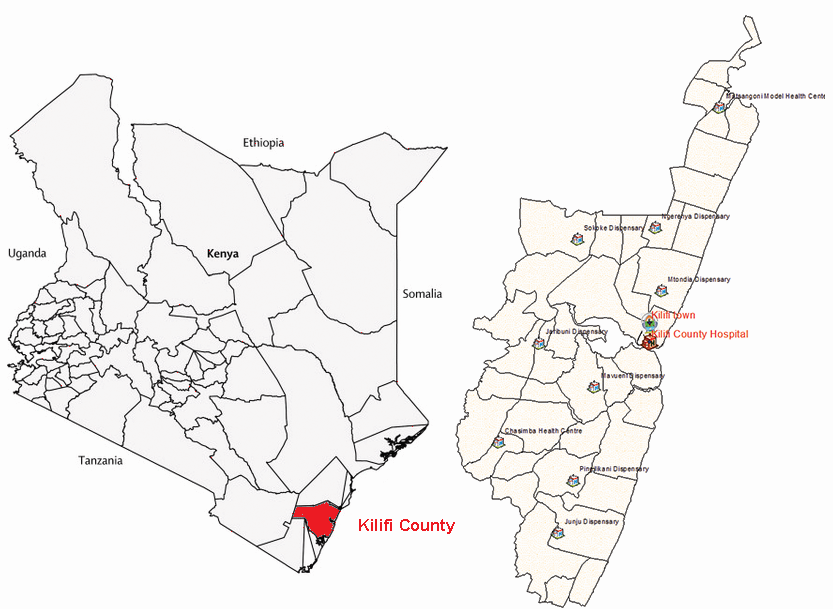
\includegraphics[keepaspectratio,height=5in]{images/kdhss.png}}
\caption{The location of ....}
\label{fig:figure1Kh}
\end{figure}

\subsection{2.2 Study Design and Data
Management}\label{study-design-and-data-management}

Lorem Ipsum is simply dummy text of the printing and typesetting
industry. Lorem Ipsum has been the industry's standard dummy text ever
since the 1500s, when an unknown printer took a galley

\subsubsection{2.2.1 Data Quality}\label{data-quality}

Lorem Ipsum is simply dummy text of the printing and typesetting
industry. Lorem Ipsum has been the industry's standard dummy text ever
since the 1500s, when an unknown printer took a galley

\subsection{2.3 Study Population}\label{study-population}

Lorem Ipsum is simply dummy text of the printing and typesetting
industry. Lorem Ipsum has been the industry's standard dummy text ever
since the 1500s, when an unknown printer took a galley

\subsubsection{2.3.1 Inclusion Criteria}\label{inclusion-criteria}

Lorem Ipsum is simply dummy text of the printing and typesetting
industry. Lorem Ipsum has been the industry's standard dummy text ever
since the 1500s, when an unknown printer took a galley

\subsubsection{2.3.2 Exclusion Criteria}\label{exclusion-criteria}

Lorem Ipsum is simply dummy text of the printing and typesetting
industry. Lorem Ipsum has been the industry's standard dummy text ever
since the 1500s, when an unknown printer took a galley

\subsection{2.4 Outcome and Explanatory
Variables}\label{outcome-and-explanatory-variables}

Lorem Ipsum is simply dummy text of the printing and typesetting
industry. Lorem Ipsum has been the industry's standard dummy text ever
since the 1500s, when an unknown printer took a galley

\subsection{2.5 Exploratory Data
Analysis}\label{exploratory-data-analysis}

Lorem Ipsum is simply dummy text of the printing and typesetting
industry. Lorem Ipsum has been the industry's standard dummy text ever
since the 1500s, when an unknown printer took a galley

\subsubsection{2.5.1}\label{section-6}

Exploratory Data Analysis 2.5.1 and include equation that is not
referenced

In general the seasonal autoregressive moving average model is defined
as;\\
\[
\begin{array}{*{20}{c}}
{\begin{array}{*{20}{c}}
\text{ARIMA}\\
{}
\end{array}}\\
{}
\end{array}\begin{array}{*{20}{c}}
{\left( {p,d,q} \right)}\\
{\begin{array}{*{20}{c}}
 \uparrow \\
{{\text{\tiny{Non seasonal}}}}
\end{array}}
\end{array}{\rm{ }}\begin{array}{*{20}{c}}
{{{\left( {P,D,Q} \right)}_s}}\\
{\begin{array}{*{20}{c}}
 \uparrow \\
\text{\tiny{seasonal}}
\end{array}}
\end{array}
\]

In general SARIMA model with period \(s\) is defined as;

\begin{equation}
\begin{matrix}
   \left( 1-{{\varphi }_{p}}L \right)  \\
   \begin{matrix}
   \uparrow   \\
   \text{NS AR(1)}  \\
\end{matrix}  \\
\end{matrix}\begin{matrix}
   \left( 1-{{\theta }_{1}}{{L}^{s}} \right)  \\
   \begin{matrix}
   \uparrow   \\
   \text{S AR(1)}  \\
\end{matrix}  \\
\end{matrix}\begin{matrix}
   \left( 1-L \right)  \\
   \begin{matrix}
   \uparrow   \\
   \text{NS D}  \\
\end{matrix}  \\
\end{matrix}\begin{matrix}
   {{\left( 1-{{L}^{s}} \right)}_{yt}}  \\
   \begin{matrix}
   \uparrow   \\
   \text{SD}  \\
\end{matrix}  \\
\end{matrix}\begin{matrix}
   =  \\
   {}  \\
\end{matrix}\begin{matrix}
   \left( 1+{{\phi }_{p}}L \right)  \\
   \begin{matrix}
   \uparrow   \\
   \text{NS AR(1)}  \\
\end{matrix}  \\
\end{matrix}\begin{matrix}
   {{\left( 1+{{\Theta }_{1}}{{L}^{s}} \right)}_{{{\ell }_{t}}}}  \\
   \begin{matrix}
   \uparrow   \\
   \text{S AR(1)}  \\
\end{matrix}  \\
\end{matrix}
\label{eq:sarima}
\end{equation}

\subsubsection{2.5.2 S}\label{s}

\subsection{2.6 Inferential Statistics}\label{inferential-statistics}

\subsubsection{2.6.1 Inferential Statistics
1}\label{inferential-statistics-1}

Include inline eqautions like this \(x+y=x+y\) \ldots{}.

\paragraph{Model Definition and include
equation}\label{model-definition-and-include-equation}

The definition of the negative binomial spatial model is

\begin{equation}
\left. {{y}_{ijt}} \right|{{\psi }_{ijt}},\underset{\scriptscriptstyle\thicksim}{\Omega }\sim{\ }\pi \left( \left. {{y}_{ijt}} \right|{{\psi }_{ijt}};\underset{\scriptscriptstyle\thicksim}{\Omega } \right)
\label{eq:binom1}
\end{equation}

\subsubsection{2.6.2 Inferential Statistics
2}\label{inferential-statistics-2}

Our outcome for objective 3 \ldots{}

\paragraph{Model Definition}\label{model-definition}

Since our outcome is binary the general distribution is; \[
{{y}_{i}}=\left\{ \begin{matrix}
   1  \\
   0  \\
\end{matrix} \right.\begin{matrix}
   \text{if there was a death}  \\
   otherwise  \\
\end{matrix}
\]

\subsubsection{2.6.3 Model assesment and goodness of
fit}\label{model-assesment-and-goodness-of-fit}

We adopted both multilevel models and Bayesian approach for model
estimation\ldots{}.

\subsection{2.9 Ethical Clearance}\label{ethical-clearance}

Ethical approval under clearance certificate number was received from
the Human Research Ethics Committee of the University of the
Witwatersrand. The certificate is in Appendix 1.

\newpage

\addtocounter{section}{2}

\section{CHAPTER 3: RESULTS}\label{chapter-3-results}

\subsection{3.1 Introduction}\label{introduction-1}

In this chapter, we show the results of the analysis of\ldots{}\ldots{}

\subsection{3.2 Exploratory Data
Analysis}\label{exploratory-data-analysis-1}

\subsection{3.2.1}\label{section-7}

Result Exploratory Data Analysis 1

\subsubsection{3.2.2}\label{section-8}

Result Exploratory Data Analysis 2

\subsection{3.3 Bivariate Analysis}\label{bivariate-analysis}

The code for the table can be generated from
\url{https://www.tablesgenerator.com/} and put between begin \{table\}
and end \{table\}

\blandscape

\begin{table}
\centering
\captionsetup{font=scriptsize}
\resizebox{\textwidth}{!}{%
\normalsize
\renewcommand{\arraystretch}{1} 


\begin{tabular}{lllllllllll}
\toprule
Variables & \multicolumn{3}{c}{Overall} & \multicolumn{3}{c}{Data1} & \multicolumn{3}{c}{Data2}  &  P-value \\
& N (total ) &    Mean &    SD (O,B,W) &N (total ) & Mean    & SD (O,B,W) & N (total )    & Mean  &    SD (O,B,W)  &    \\
\midrule
Age & 3114 (7820) & 35.95 & 32.56 & 3114 (7621) & 35.71 & 32.35 & 199 ( 199) & 45.16 & 38.69 & 0.0001 \\
 &  &  & 28.53 &  &  & 28.48 &  &  & 38.69 &  \\
 &  &  & 14.73 &  &  & 14.46 &  &  & N/A &  \\
 \midrule
 Days & 3113 (7780) & 5.18 & 6.61 & 3113 (7591) & 5.15 & 6.53 & 189 ( 189) & 6.51 & 9.16 & 0.0067 \\
 &  &  & 4.95 &  &  & 5.04 &  &  & 9.16 &  \\
 &  &  & 4.45 &  &  & 4.34 &  &  & N/A &  \\
 \midrule
Number of  & 3114 (7820) & 3.49 & 2.56 & 3114 (7621) & 3.50 & 2.58 & 199 ( 199) & 2.96 & 1.75 & 0.0036 \\
 &  &  & 1.59 &  &  & 1.59 &  &  & 1.75 &  \\
 &  &  & N/A &  &  & N/A &  &  & N/A &  \\
 \midrule
Total  & 3114 (7820) & 3.22 & 2.27 & 3114 (7621) & 3.23 & 2.29 & 199 ( 199) & 2.67 & 1.37 & 0.0007 \\
 &  &  & 1.37 &  &  & 1.37 &  &  & 1.37 &  \\
 &  &  & N/A &  &  & N/A &  &  & N/A &  \\
 \midrule
Weight  & 3109 (7736) & 10.96 & 5.17 & 3108 (7541) & 10.97 & 5.13 & 195 ( 195) & 10.53 & 6.38 & 0.2597 \\
 &  &  & 4.69 &  &  & 4.68 &  &  & 6.38 &  \\
 &  &  & 2.16 &  &  & 2.13 &  &  & N/A &  \\
 \midrule
Height  & 3092 (7526) & 85.17 & 19.06 & 3088 (7350) & 85.12 & 18.98 & 176 ( 176) & 87.05 & 22.45 & 0.1939 \\
 &  &  & 17.09 &  &  & 17.14 &  &  & 22.45 &  \\
 &  &  & 8.53 &  &  & 8.40 &  &  & N/A &  \\
\midrule
Water (mm) & 3070 (7426) & 31.92 & 44.30 & 3068 (7236) & 31.78 & 44.02 & 190 ( 190) & 37.27 & 53.79 & 0.1002 \\
 &  &  & 32.42 &  &  & 32.78 &  &  & 53.79 &  \\
 &  &  & 32.84 &  &  & 32.30 &  &  & N/A & \\
\bottomrule
\end{tabular}%
}


\caption{Characteristics of the study population for the continous variables a bivariate analysis by mortality; SD(O,B,W)  is the overall, within and between Standard Deviation}
\label{tab:table1}
\end{table}

\elandscape

\subsection{3.4 Inferential 1 Model Fit and
Diagnostics}\label{inferential-1-model-fit-and-diagnostics}

\subsubsection{3.4.1 Model fit results}\label{model-fit-results}

orem Ipsum is simply dummy text of the printing and typesetting
industry. \#\#\# 3.4.2 Model fit diagnostics orem Ipsum is simply dummy
text of the printing and typesetting industry.

\subsection{3.5 Inferential 2 Model Fit and
Diagnostics}\label{inferential-2-model-fit-and-diagnostics}

\subsubsection{3.5.1 Model fit results}\label{model-fit-results-1}

orem Ipsum is simply dummy text of the printing and typesetting
industry.

\subsubsection{3.5.2 Model fit diagnostics}\label{model-fit-diagnostics}

orem Ipsum is simply dummy text of the printing and typesetting
industry.

\addtocounter{section}{3}\newpage

\section{CHAPTER 4: DISCUSSION AND
CONCLUSION}\label{chapter-4-discussion-and-conclusion}

\subsection{4.1 Introduction}\label{introduction-2}

This chapter discusses the key results from our analysis

In general, reference Figure\textasciitilde{}\ref{fig:figure1}.

\subsection{4.2}\label{section-9}

Lorem Ipsum is simply dummy text of the printing and typesetting
industry

\subsection{4.3}\label{section-10}

Lorem Ipsum is simply dummy text of the printing and typesetting
industry \#\# 4.4 Lorem Ipsum is simply dummy text of the printing and
typesetting industry

\subsection{4.5 Strengths and limitations of the
study}\label{strengths-and-limitations-of-the-study}

The strength and limitations of the results and discussion in this
research project are discussed in four broad categories;

\begin{itemize}
\tightlist
\item
  Category 1
\item
  Category 2
\end{itemize}

\subsubsection{4.5.1 Category 1}\label{category-1}

.Lorem Ipsum is simply dummy text of the printing and typesetting
industry

\subsubsection{4.5.2 Category 2}\label{category-2}

Lorem Ipsum is simply dummy text of the printing and typesetting
industry

\subsection{4.6 Conclusion}\label{conclusion}

in conclusion \ldots{}..

\addtocounter{section}{5}

\newpage

\section{REFERENCES}\label{references}

\small 

\hypertarget{refs}{}
\hypertarget{ref-Black2013}{}
1. Kazembe LN, Chirwa TF, Simbeye JS, Namangale JJ. Applications of
bayesian approach in modelling risk of malaria-related hospital
mortality. BMC Medical Research Methodology. 2008;8:6.

\hypertarget{ref-Black2008}{}
2. Greenspan J, Bulger B. MySQL/php database applications
{[}Internet{]}. John Wiley \& Sons, Inc. 2001 {[}cited 2017 Jun 6{]}.
Available from: \url{http://dl.acm.org/citation.cfm?id=558011}

\section{APPENDICES}\label{appendices}

\subsection{Appendix 1 - Plagiarism declaration
report}\label{appendix-1---plagiarism-declaration-report}


\includegraphics{../docs/plagiarism_doc.pdf}

\addtocounter{section}{4}

\subsection{Clearance Certificate}\label{clearance-certificate}


\includegraphics{../docs/ethics_certificate.pdf}


\end{document}
